\documentclass[12pt,letterpaper]{article}
\usepackage{slashbox}
\usepackage{pgf}
\usepackage{amsmath,amsthm,amsfonts,amssymb,amscd}
\usepackage{fullpage}
\usepackage{lastpage}
\usepackage{enumerate}
\usepackage{fancyhdr}
\usepackage{mathrsfs}
\usepackage{xcolor}
\usepackage{float}
\usepackage[margin=2cm]{geometry}
\geometry{
 a4paper,
 total={210mm,297mm},
 left=20mm,
 right=20mm,
 top=20mm,
 bottom=20mm,
 }
\setlength{\parindent}{0.0in}
\setlength{\parskip}{0.05in}
\renewcommand{\headrulewidth}{0pt}
\renewcommand{\footrulewidth}{0pt}

% Edit these as appropriate
\newcommand\course{CS6097}
\newcommand\coursename{Wireless Net}
\newcommand\semester{Fall 2014}     % <-- current semester
\newcommand\hwnum{4}                  % <-- homework number
\newcommand\yourname{Chris Park (Kyungmook)} % <-- your name
\newcommand\login{M07068980}           % <-- your NetID
\newcommand\hwdate{Due: Oct 1st 2014 6:00PM} % <-- HW due date
\newcommand\problems{P1.19, P6.5, P6.8, P6.13, P6.17}
\newenvironment{answer}[1]{
  \subsubsection*{Problem #1}
}


\pagestyle{fancyplain}
%\setlength{\headheight}{72pt}
%\chead{\textbf{\Large{Homework \hwnum}}}
%\rhead{\yourname\ \login\\\course\coursename\ --- \semester\\\hwdate\\\problems\\}
%\headsep 50pt


\begin{document}

\begin{flushright}
\yourname\ \login\\\course\coursename\ --- \semester\\\hwdate\\\problems\\
\end{flushright}

\begin{center}
\textbf{\Large{Homework \hwnum}}
\end{center}

\begin{answer}{1}

\textbf{{P1.19: } If a total of 33 MHz of bandwidth is allocated to a particular cellular telephone system which uses two 25 kHz simplex channels to provide full duplex voice channels, compute the number of simultaneous calls that can be supported per cell if a system uses:}

\begin{enumerate}[(a)]
\item
\textbf{FDMA}\\
FDMA requires single channel per carrier. If the cellular telephone system uses two 25 kHz simplex channels, each call would require 50 kHz of bandwidth. Therefore, the number of simultaneous calls that can be supported per cell is $\frac{33 MHz}{50 kHz} =$ \framebox[1.1\width]{660 calls}\\

\item
\textbf{TDMA with 8-way time multiplexing}\\
This type of TDMA can utilize 8-way time multiplexing to employ 8 users per 50 kHz of allocated bandwidth. This means it can serve 8 times to the number of calls that the previous FDMA can serve. Therefore, the number of simultaneous calls that can be supported per cell is $660\;calls \times 8 =$ \framebox[1.1\width]{5280 calls}\\
\end{enumerate}

\end{answer}

\begin{answer}{2}
\flushleft
\textbf{{P6.5: } In a given system with shared access, the probability of “n” terminals communicating at the same time is given by\\
\centering
$p(n)=\frac{(1.5G)^ne^{-1.5G}}{(n-1)!}$\\
\flushleft
where G is the traffic load in the system. What is the optimal condition for $p$?}\\

It is desirable to reduce to number of n terminals connecting at the same time to be equal to G, the traffic load in the system. Then, the carrier can maximize the use of the system without having to drop calls.\\

Therefore, the optimal condition for p is: \framebox[1.1\width]{$p(G)=\frac{(1.5G)^ne^{-1.5G}}{(G-1)!}$}\\

\end{answer}

\begin{answer}{3}

\textbf{{P6.8: } Can we use CSMA/CD in cellular wireless networks? Explain your answer with solid reasons.}\\

No, we can't use CSMA/CD in cellular wireless networks. CSMA/CD reduces the effect of a collision as it renders the medium ready to be used as soon as possible in wired Ethernet. In wireless networks, since we can either transmit or receive data using the radio, it is not possible to transmit and receive data at the same time to detect collisions in a shared channel.\\

\end{answer}

\begin{answer}{4}

\textbf{{P6.13: } What in your opinion should be the criteria to select the value of the contention window? Also explain how you will decide the value of the time slot for CSMA/CA.}\\
 
The goal of the contention window is to avoid collision by assigning enough time to each terminal before it starts transmitting data. The contention window will depend on how often and long the medium stays busy, i.e. the traffic load on a system. Depending on the severity of the traffic, the system would have to assign larger margin of contention window to avoid collision. The backoff counter that counts down in the contention window is frozen when the medium is busy. It starts counting down once the medium stays idle for time that exceeds the distributed interframe space.\\

I will choose the time slot based on the IEEE standards. For example, if the wireless device follows the IEEE 802.11g standard, I will choose the value between 9$\mu{s}$ to 20$\mu{s}$ depending on the traffic information that device is utilized.\\

For example, I will start with 9$\mu{s}$ and collect how many collisions occurred within two hours. I will increase the slot time by 1$\mu{s}$ and repeat the experiment until 20$\mu{s}$, which will provide data that allows us to run a statistical analysis and determine which time slot is the most effect for the environment that the device is operating in.\\

\end{answer}

\begin{answer}{5}

\textbf{{P6.17: } Suppose the propagation delay is $\alpha$, SIFS is $\alpha$, DIFS is 3$\alpha$, and RTS and CTS are 5$\alpha$, respectively, for CSMA/CA with RTS/CTS.}\\

\begin{figure}[H]
\centering
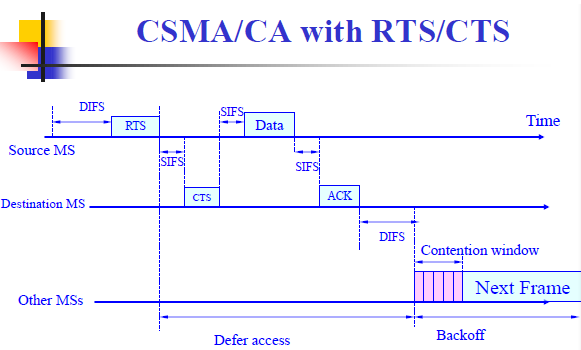
\includegraphics[width=5in]{CSMACAwithRTSCTS.png}
\caption{CSMA/CA with RTS/CTS}
\end{figure}
\flushleft

\begin{figure}[H]
\centering
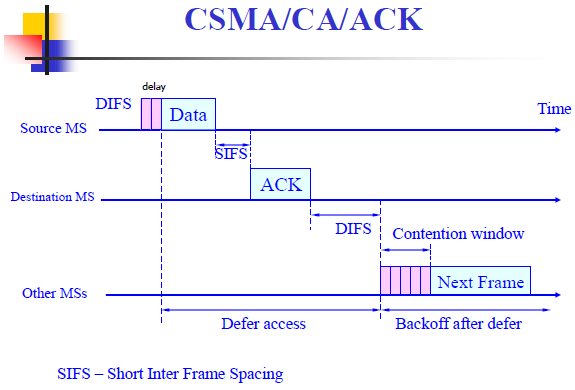
\includegraphics[width=5in]{CSMACAwithACK.png}
\caption{CSMA/CA with ACK}
\end{figure}
\flushleft

\begin{enumerate}[(a)]
\item
\textbf{What is the earliest time for the receiver to send the CTS message?}\\



Transmitter sends an RTS after medium has been idle for more than DIFS, RTS, and SIFS as shown in Figure 1.\\
$\therefore$ The earliest time to send CTS message = $DIFS+RTS+Propagation Delay+SIFS = 3\alpha+5\alpha+\alpha+\alpha = 10\alpha$\\

\item
\textbf{If the data packet is 100$\alpha$ long, what is the shortest time for the receiver to send the ACK signal?}\\

As shown in Figure 2, the shortest time to send the ACK signal = $DIFS+Propagation Delay+Data+SIFS=3\alpha+\alpha+100\alpha+\alpha=105\alpha$

\item
\textbf{Explain why SIFS is kept smaller than DIFS.}\\

SIFS exists to ensure the full transfer of data, a data fragment burst. It doesn't need to be as long as the DIFS. It needs to be long enough to ensure the data transfer is complete, so that the ACK signal can be sent afterward. IEEE 802.11-9.2.3.1 states SIFS is the shortest of the interframe spaces. SIFS shall be used when STAs have seized the medium and
need to keep it for the duration of the frame exchange sequence to be performed. Using the smallest gap between transmissions within the frame exchange sequence prevents other STAs, which are required to wait for the medium to be idle for a longer gap, from attempting to use the medium, thus giving priority to completion of the frame exchange sequence in progress.\\

\item
\textbf{Can you make SIFS = 0?}\\

No, in case where ACK signal has a collision, causing the device to not receive the ACK signal, the data frame is presumed to be lost. Also, SIFS ensures that the Data is fully transmitted. Without it, ACK signal may be sent with data corrupt.
\end{enumerate}



\end{answer}

\end{document}
